\documentclass[11pt]{article}

\usepackage{amssymb}
\usepackage{amsmath, esint}
\usepackage{amsthm}
\usepackage{array}
\usepackage{longtable}
\usepackage{mathtools}
\usepackage{pdfpages}
\usepackage{fancyhdr}
\usepackage[figurename=Figure]{caption}
\usepackage{empheq}
\usepackage{mdframed}
\usepackage[a4paper, left=1in,right=1in,top=1in,bottom=0.7in,footskip=0.6in,includeheadfoot]{geometry}
\usepackage{tikz}
\usepackage{pgfplots}
\usepackage{hyperref}
\usepackage{wrapfig}
\usepackage{enumitem}
\usepackage{lastpage}
\usepackage{zref-totpages}

%title
\edef\mytitle{Precalculus}
\edef\mysubtitle{Lesson 4: Transcendental Functions}
\edef\mydate{June 25, 2024}
\edef\myauthor{Tyler Wang}

\usetikzlibrary{calc, backgrounds,angles, quotes}

\tikzset{
    partial ellipse/.style args={#1:#2:#3}{
        insert path={+ (#1:#3) arc (#1:#2:#3)}
    }
}

\setlength{\parskip}{10pt}
\setlength{\parindent}{0pt}

\fancyhf{}
\fancyfoot[l]{\copyright \,\,\myauthor}
\fancyhead[L]{\mysubtitle}
\fancyhead[r]{\mytitle}
\fancyfoot[c]{Page \thepage \hspace{1pt} of \ztotpages}
\pagestyle{fancy}

\fancypagestyle{plain}{
\fancyhf{}
\fancyfoot[l]{\copyright \,\,\myauthor}
\fancyfoot[c]{Page \thepage \hspace{1pt} of \ztotpages}
\renewcommand{\headrulewidth}{0pt}}

\newmdtheoremenv{lemma}{Lemma}
\newmdtheoremenv{prop}{Proposition}
\newmdtheoremenv{define}{Definition}
\newmdtheoremenv{theorem}{Theorem}
\newmdtheoremenv{cor}{Corollary}

\numberwithin{lemma}{section}
\numberwithin{equation}{section}
\numberwithin{define}{section}
\numberwithin{prop}{section}
\numberwithin{figure}{section}
\numberwithin{theorem}{section}
\numberwithin{cor}{section}

\newcounter{ex}[section]
\newenvironment{ex}[0]{

	\refstepcounter{ex}
    \subsection*{Example \theex .}
    }
    {
    \subsection*{}
    }
\numberwithin{ex}{section}

\def\real{\mathbb{R}}
\def\complex{\mathbb{C}}
\def\rat{\mathbb{Q}}
\def\nat{\mathbb{N}}
\def\integ{\mathbb{Z}}
\def\mod#1{\mathbb{Z}_{#1}}
\def\cpx{\mathbb{C}}

\def\paren#1{\left(#1\right)}
\def\sbrak#1{\left[#1\right]}
\def\cbrak#1{\left\{#1\right\}}

\def\ceil#1{\left\lceil #1 \right\rceil}
\def\floor#1{\left\lfloor #1 \right\rfloor}
\def\abs#1{\left\lvert #1 \right\rvert}
\def\abrak#1{\left\langle #1 \right\rangle}
\def\bra#1{\left\langle #1 \right\rvert}
\def\ket#1{\left\lvert #1 \right\rangle}
\def\braket#1#2{\left\langle #1 \left.\right\lvert #2 \right\rangle}

\def\jand{\quad\text{and}\quad}
\def\jor{\quad\text{or}\quad}
\def\for{\quad\text{for }\,}

\def\ieval#1#2{\Bigg|^{#2}_{#1}}
\def\deval#1{\bigg|_{#1}}

\def\diff#1#2{\frac{d#1}{d#2}}
\def\pdiff#1#2{\frac{\partial#1}{\partial#2}}

\def\sec#1{\section*{#1}\addtocounter{section}{1}\setcounter{subsection}{0}}

\hypersetup{
    colorlinks=true,
    urlcolor=blue,
    linkcolor=magenta,
    pdfborderstyle={/S/U/W 1}
}

\setlength\extrarowheight{3pt}

\title{\mytitle \\ [2ex] \Large \mysubtitle}
\date{\small Modified \mydate}
\author {Tyler Wang\thanks{
\href{mailto:wangtyler123@gmail.com}{wangtyler123@gmail.com}}}

\begin{document}
\maketitle
\section{Exponentials}
\subsection{Exponentials for Reals}
Before we dive into this topic, we must define the idea of taking an exponential, with the domain being the real numbers. Traditional exponentials have the disadvantage of only working with integer values or rational numbers.
However, the problem is that the rational numbers are only a very small subset of the set of real numbers.\footnote{
The set of rational numbers is so small that the entire set doesn't even take up "space" in the real numbers. It is what's called a \textit{\href{https://en.wikipedia.org/wiki/Null_set}{null set}.}}
So for our purposes, we need something a little better.
For our definition, we'd like to seek a nice connected function that outputs the same values as the discrete exponent and also satisfies all of the properties that the discrete case does.
Unfortunately, this definition is quite a calculus heavily so I will leave that discussion for another class. For our class, we will only so we will only look over a few of its properties.
\begin{theorem}
Let $x,y\in\real$, and $a\in\real^{+}$ then the following hold:
\begin{enumerate}
	\item $a^xb^y=a^{a+b}$
	\item $(a^x)^y=a^{xy}$
	\item for $b\in\real$, $(ab)^x=a^xb^x$
\end{enumerate}
(\textbf{Note}: the exponential is only defined for $a$ that is positive)
\end{theorem}

We can in fact verify these properties quite easily if we shrink the domain to just the rational numbers. I will leave this as an exercise for the reader.

\begin{figure}[h]
	\centering
	\begin{tikzpicture}
		\begin{axis}
			\addplot[thick, color=blue, samples=100]{exp(x)};
		\end{axis}
	\end{tikzpicture}
	\caption{}
	\label{fig:exp}
\end{figure}

If we decide to plot the exponential function, we notice in figure \eqref{fig:exp} that the exponential is defined for all real numbers, but as the input gets smaller and smaller, it seems to \textit{approach} zero. We call this a \textbf{horizontal asymptote} and claim there's a horizontal asymptote for the function $a^x$ when $x$ approaches $-\infty$. Since the function never reaches zero, we claim the domain and image for the exponential function is
$$\mathcal{D}=\real \jand a^\mathcal{D}=(0,+\infty).$$

\subsection{Inverse of Exponential (Logarithm)}
\begin{define}
	Let $f(x)=a^x$. Then $f^{-1}(x)=log_a(x)$ read "log base $a$ of $x$".\footnotemark
\end{define}
\begin{figure}[h]
	\centering
	\begin{tikzpicture}
		\begin{axis}
			\addplot[thick, color=blue, domain=-10:10, samples=100]{ln(x)};
		\end{axis}
	\end{tikzpicture}
	\caption{}
	\label{fig:log}
\end{figure}
\footnotetext{When you see a log without a subscript, it can mean one of two things depending on context. In general, this will mean $log_{10}$, since this is used often when plotting data that grows exponentially. In a more mathematical context, this will generally mean natural log, which we will discuss later.}
As you can see in figure \eqref{fig:log}, the logarithm is defined for all $x\in(0,\infty)$. We can observe there is a \textbf{vertical asymtote} at $0$.
Since as far as we are concerned, the image of $a^x$ doesn't include negative numbers, the logarithm is not defined for $(-\infty,0]$.

Now we have the definition of the logarithm, let's look at some of its properties.
\begin{theorem}
	Let $x,y\in\real$, and $a\in\real^{+}$ then the following hold:
	\begin{enumerate}
		\item $\log_a(x)+\log_a(y)=\log_a(xy)$
		\item $y\log_a(x)=\log_a(x^y)$
	\end{enumerate}
\end{theorem}
\begin{proof}
	Since
	$$a^{\log_a(xy)}=xy=a^{\log_a(x)}a^{\log_a(y)}=a^{\log_a(x)+\log_a(y)}.$$
	Then taking the logarithm of both sides gives
	$$\log_a(a^{\log_a(xy)})=\log_a(a^{\log_a(x)+\log_a(y)})$$
	$$\log_a(xy)=\log_a(x)+\log_a(y).$$
	hence proving (1).

	Then since
	$$a^{y\log_a(x)}=x^y=a^{\log(x^y)}$$
	Taking the logarithm of both sides:
	$$\log_a(a^{y\log_a(x)})=\log_a(a^{\log(x^y)})$$
	$$y\log_a(x)=\log(x^y).$$
	Hence proving (2).
\end{proof}

\subsection{Change of Basis}
\begin{theorem}
Let $a,b\in(0,\infty)$ and $x\in\real$. Then
$$a^x=b^{\log_b(a)x}$$
\label{thm:changeofexp}
\end{theorem}
\begin{proof}
	Since $a=b^{\log_b(a)}$, using the properties the exponential,
	$$a^x=(b^{\log_b(a)})^x=b^{\log_b(a)x}$$
	hence proving the theorem.
\end{proof}

\begin{theorem}
	Let $a,b\in(0,\infty)$ and $x\in\real$. Then
	$$\log_a(x)=\frac{\log_b(x)}{\log_b(a)}$$

	\label{thm:changeoflog}
\end{theorem}
\begin{proof}
	By the definition of the logarithm, $\log_a(x)$ implies
	$$a^{\log_a(x)}=b^{\log_b(a)\log_a(x)}=x$$
	since $a=b^{\log_b(a)}$.
	Taking the $\log_b$ on both sides gives
	$$\log_b(b^{\log_b(a)\log_a(x)})=\log_b(x)$$
	hence
	$$\log_b(a)\log_a(x)=\log_b(x)$$
	implying
	$$\log_a(x)=\frac{\log_b(x)}{\log_b(a)}$$
\end{proof}

What theorems \eqref{thm:changeofexp} and \eqref{thm:changeoflog} tell us is that we can write any exponential as an exponential function of any other base.

The utility of theorems \eqref{thm:changeofexp} and \eqref{thm:changeoflog} might not be immediately clear, so let's discuss it here.
Like $\pi$, there is a number $e\approx 2.71828$ which is also irrational that we often use in the context of exponentials. $e$ can be thought of as a preferred basis when working with exponentials, due to its special properties.
We will not discuss the special properties of this number, since it relates heavily to calculus, but we will introduce the notation to get you familiar with the idea.
For example, using theorem \eqref{thm:changeofexp}, we can write the function
$$f(x)=2^x$$
as
$$f(x)=e^{\log_e(x)x}$$
Because of how fundamental $e^x$ is in the context of exponentials, we give it a special name: $\exp(x)$ (where exp stands for exponential).
The advantage of this notation is that sometimes, with longer arguments, it's a little easier to read, but it also highlights that although similar, the $\real$ exponential and the discrete version are distinct mathematical operations.
Additionally, we also define a special function for $\log_e(x)$ called $\ln(x)$, or natural logarithm (or \textit{logarithme naturel}  in French).

Although we started by defining an exponential with an arbitrary base, in modern mathematics, we first define $\exp(x)$ (or $\ln(x)$) since we view $e^x$ and $\ln(x)$ as more fundamental than an exponential with an arbitrary base (hence why its called \textit{natrual} log). Hopefully, in a future math class, the reason for this will become clearer, but for this class, we will end our discussion here.

\section{Trignometry}
\subsection{Definition}
 Now we have come to everyone's favorite topic, trig. But before, we get into this topic, we must define our functions.
 	\begin{define}
 		\label{def:trigdefine}
		Using the figure below, let $\odot\,O$ be a unit circle (radius 1), then for any $\theta\in\real$ (measuring counterclockwise from $+x$ axis if $\theta$ is positive, and clockwise if $\theta$ is negative)
		$$x=\cos(\theta) \jand y=\sin(\theta)\footnotemark$$
		\begin{center}
			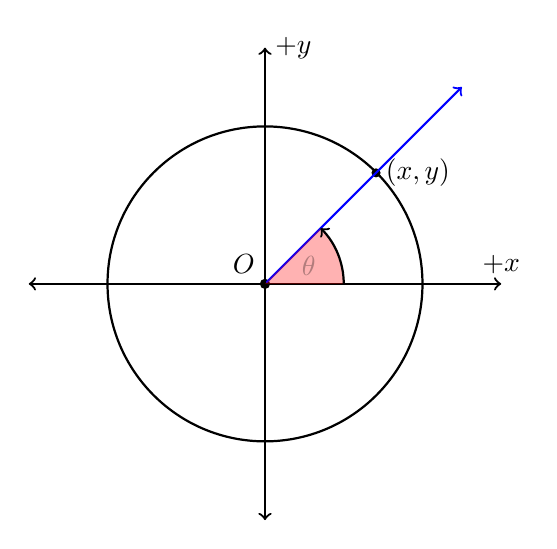
\begin{tikzpicture}
 				\draw[thick,black] (0,0) circle (2);
 				\filldraw[thick,black] (0,0) coordinate (O) circle (0.05) node[above left] {$O$};

 				\filldraw (1.41,1.41) coordinate (A) circle (0.05) node[right] {$(x,y)$};

 				\draw[thick,blue,->] (0,0) -- (2.5,2.5) ;

 				\draw[thick,<->] (-3,0) -- (3,0) coordinate (B) node[above] {$+x$};
 				\draw[thick,<->] (0,-3) -- (0,3) node[right] {$+y$};

 				\draw pic["$\theta$", draw,->, black, thick, fill=red, fill opacity=0.3, angle radius=1cm] {angle = B--O--A};
			\end{tikzpicture}
	\end{center}
\end{define}

\footnotetext{Check this is the same definition as \textit{"SOHCAHTOA"}.}

Then using definition \eqref{def:trigdefine}, we can define the other trig functions in the conventional manner:
$$\tan(x)=\frac{\sin(x)}{\cos(x)}
\for x\in \cbrak{x\in\real: x\neq \frac{\pi}{2}+\pi n, \:
\forall n\in\nat}$$
$$\cot(x)=\frac{\cos(x)}{\sin(x)}
\for \cbrak{x\in\real :x\neq\pi n, \:
\forall n\in\nat}$$
$$\csc(x)=\frac{1}{\sin(x)} \for \cbrak{x\in\real :x\neq\pi n, \:
\forall n\in\nat}$$
$$\text{sec}(x)=\frac{1}{\cos(x)}
\for x\in \cbrak{x\in\real: x\neq \frac{\pi}{2}+\pi n, \:
\forall n\in\nat}$$

Then to find the image, trivially from the definition \eqref{def:trigdefine}, $|\sin(x)|,|\cos(x)\le 1$, hence the image of $\sin(x)$ and $\cos(x)$ is the interval $[-1,1]$.
Then immediately, since $\csc(x)$ and $\text{sec}(x)$ are just the recipricals of $\sin(x)$ and $\cos(x)$ respectivly, $|\csc(x)|,|\text{sec}(x)|\ge 1$ hence the image these functions is the compound interval $[-\infty,-1]\cup[1,\infty]$.

Finding the image of $\tan(x)$ and $\cot(x)$ can be a bit more tricky, but we will leverage a computer to help us do this. Using figures \eqref{fig:tan} and \eqref{fig:cot}, we see the image of our two functions is $\real$.
\begin{figure}[h]
	\centering
	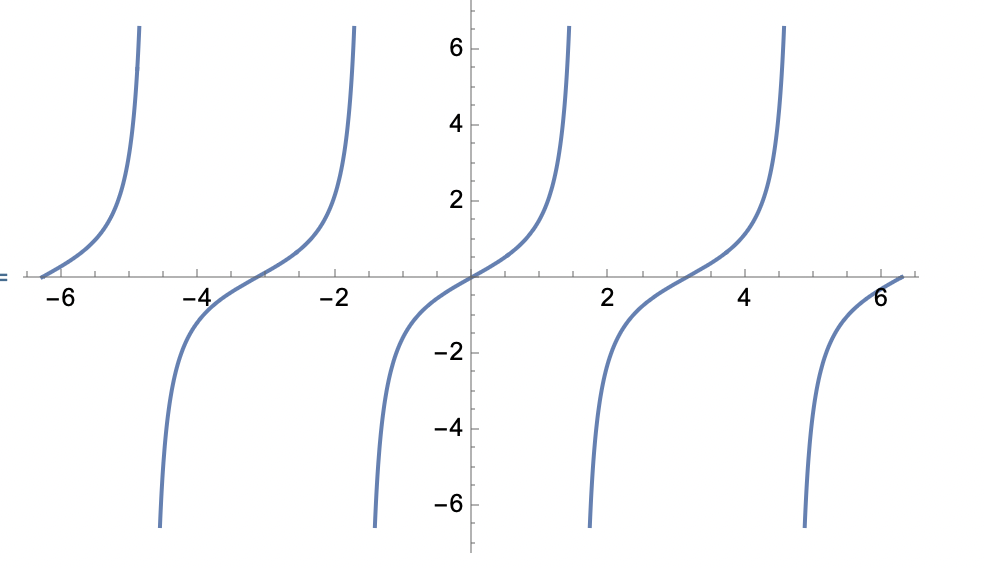
\includegraphics[scale=0.6]{assets/Lesson5/tanplot.png}
	\caption{Plot of $\tan(x)$}
	\label{fig:tan}
\end{figure}
\begin{figure}[h]
	\centering
	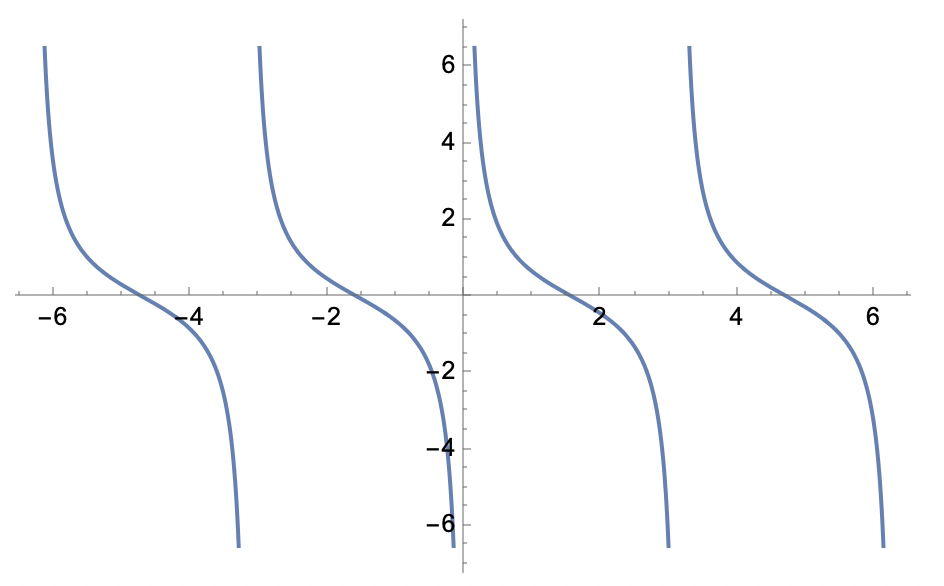
\includegraphics[scale=0.6]{assets/Lesson5/cotplot.png}
	\caption{Plot of $\cot(x)$}
	\label{fig:cot}
\end{figure}

\subsection{Basic Identities}
\subsubsection{Trig Function Identities}
\begin{theorem}
\label{thm:perod}
$\sin(x)$ and $\cos(x)$ are $2\pi$ periodic, or equivalently,
$$\sin(x)=\sin(x+2\pi) \jand \cos(x)=\cos(x+2\pi)$$
\end{theorem}
\begin{proof}
	Since $\sin(x)$ $\cos(x)$ are defined on the unit circle, the angle can be represented $x$ can be more generally written as
	$$x+2\pi k \for k\in\integ$$
	Hence
	$$\sin(x+2\pi k)=\sin(x) \jand
	\cos(x+2\pi k)=\cos(x)$$
	hence proving the theorem.
\end{proof}

\begin{cor}
	$\text{sec}(x)$, $\csc(x)$ are $2\pi$ periodic.
\end{cor}
\begin{proof}
	This proof is trivial with theorem \eqref{thm:perod}.
\end{proof}

\begin{theorem}
$\tan(x)$, $\cot(x)$ are $\pi$ periodic
\label{thm:tanperodic}
\end{theorem}
\begin{proof}
	Postponed for a later section.
\end{proof}

\begin{theorem}
	$\sin(x)$ is odd.
	\label{thm:sinodd}
\end{theorem}
\begin{proof}
	Let's prove this statement first only for the domain $[-\pi,\pi]$.
	For an angle $\theta$, since $-\theta$ is the same angle reflected over the x-axis, by this reflection and definition \eqref{def:trigdefine},
	$$\sin(x)=-\sin(-x)$$
	Then by theorem \eqref{thm:perod},
	$$\sin(x)=\sin(x+2\pi k)=-\sin(-x)=-\sin(-x+2\pi m)$$
	for arbitrary $k,m\in\integ$. Then since these constants are arbitrary, let $k=-m$, hence
	$$\sin(x+2\pi k)=-\sin(-x-2\pi k)$$
	which implies
	$$\sin(x+2\pi k)=-\sin(-(x+2\pi k))$$
	Since $x+2\pi k$ covers the entire set $\real$, we conclude that $\sin(x)$ is odd over $\real$.
\end{proof}

\begin{theorem}
	$\cos(x)$ is even.
	\label{thm:coseven}
\end{theorem}
\begin{proof}
	Following very closely to the previous proof, let's prove this statement first only for the domain $[-\pi,\pi]$.
	For an angle $\theta$, since $-\theta$ is the same angle reflected over the x-axis, by this reflection and definition \eqref{def:trigdefine},
	$$\cos(x)=\cos(-x)$$
	Then by theorem \eqref{thm:perod},
	$$\cos(x)=\cos(x+2\pi k)=\cos(-x)=\cos(-x+2\pi m)$$
	for arbitrary $k,m\in\integ$. Then since these constants are arbitrary, let $k=-m$, hence
	$$\cos(x+2\pi k)=\cos(-x-2\pi k)$$
	which implies
	$$\cos(x+2\pi k)=\cos(-(x+2\pi k))$$
	Since $x+2\pi k$ covers the entire set $\real$, we conclude that $\cos(x)$ is even over $\real$.
\end{proof}

\begin{cor}
	$\tan(x)$,$\cot(x)$,$\csc(x)$ are odd, and $\text{sec}(x)$ is even.
\end{cor}
\begin{proof}
	Exercise.
\end{proof}



\subsubsection{Pythagorean-esque Identies}
\begin{theorem}[Pythagorean Identity]
\label{thm:pydi}
Let $x\in\real$, then
$$\cos^2(x)+\sin^2(x)=1$$
\end{theorem}
\begin{proof}
	By definition \eqref{def:trigdefine}, the ordered pair $(\cos(x),\sin(x))$ lies on a unit circle. Therefore since a circle satisfies the relation
	$$x^2+y^2=1$$
	it immediately follows that
	$$\cos^2(x)+\sin^2(x)=1$$
\end{proof}
\begin{cor}
Let $x\in \cbrak{x\in\real: x\neq \frac{\pi}{2}+\pi n, \:
\forall n\in\nat}$, then
$$\text{sec}^2(x)=1+\tan^2(x)$$
\end{cor}
\begin{proof}
	Using theorem \eqref{thm:pydi},
	$$\cos^2(x)+\sin^2(x)=1$$
	Since $\cos(x)\neq0$ by our domain restriction,
	$$1+\frac{\sin^2(x)}{\cos^2(x)}=\frac{1}{\cos^2(x)}=\text{sec}^2(x)$$
	hence
	$$1+\tan^2(x)=\text{sec}^2(x).$$
\end{proof}

\begin{cor}
	Let $x\in \cbrak{x\in\real: x\neq \pi n, \:
\forall n\in\nat}$, then
$$\csc^2(x)=1+\cot^2(x)$$
\end{cor}
\begin{proof}
	Using theorem \eqref{thm:pydi},
	$$\cos^2(x)+\sin^2(x)=1$$
	Since $\sin(x)\neq0$ by our domain restriction,
	$$\frac{\cos^2(x)}{\sin^2(x)}+1=\frac{1}{\sin^2(x)}=\csc^2(x)$$
	hence
	$$1+\cot^2(x)=\csc^2(x).$$
\end{proof}

\subsubsection{Angle Identies}
\begin{theorem}
\label{thm:sumcos}
For $\alpha,\beta\in\real$,
$$\cos(\alpha+\beta)=\cos(\alpha)\cos(\beta)-\sin(\alpha)\sin(\beta)$$
\end{theorem}
\begin{proof}
	Postponed indefinitely.
\end{proof}
\begin{cor}
	For $\alpha,\beta\in\real$,
$$\cos(\alpha-\beta)=\cos(\alpha)\cos(\beta)+\sin(\alpha)\sin(\beta)$$
\end{cor}
\begin{proof}
	Using theorems \eqref{thm:coseven} and \eqref{thm:sinodd},
	$$\cos(\alpha-\beta)=
	\cos(\alpha)\cos(-\beta)-\sin(\alpha)\sin(-\beta)=
	\cos(\alpha)\cos(\beta)+\sin(\alpha)\sin(\beta)$$
\end{proof}

\begin{theorem}
\label{thm:sumsin}
For $\alpha,\beta\in\real$,
$$\sin(\alpha+\beta)=\sin(\alpha)\cos(\beta)+\cos(\alpha)\sin(\beta)$$
\end{theorem}
\begin{proof}
	Postponed indefinitely.
\end{proof}

\begin{cor}
	For $\alpha,\beta\in\real$,
$$\sin(\alpha-\beta)=\sin(\alpha)\cos(\beta)-\cos(\alpha)\sin(\beta)$$
\end{cor}
\begin{proof}
	Using theorems \eqref{thm:coseven} and \eqref{thm:sinodd},
	$$\sin(\alpha-\beta)=\sin(\alpha)\cos(-\beta)+\cos(\alpha)\sin(-\beta)
	=\sin(\alpha)\cos(\beta)-\cos(\beta)\sin(\beta)$$
\end{proof}

\begin{cor}[Double angle]
	For $\theta\in\real$, the following are true:
	$$\sin(2\theta)=2\sin(\theta)\cos(\theta)$$
	$$\cos(2\theta)=\cos^2(\theta)-\sin^2(\theta)$$
	\label{cor:doubleangle}
\end{cor}
\begin{proof}
	Trivial by theormes \eqref{thm:sumcos} and \eqref{thm:sumsin}.
\end{proof}

\begin{cor}[Half angle]
	For $\theta\in\real$, the following are true:
	$$\sin\paren{\frac{\theta}{2}}=\pm\sqrt{\frac{1-\cos(\theta)}{2}}$$
	$$\cos\paren{\frac{\theta}{2}}=\pm\sqrt{\frac{1+\cos(\theta)}{2}}$$
\end{cor}
\begin{proof}
	Using corrolary \eqref{cor:doubleangle} and letting $x=\frac{\theta}{2}$ gives
	$$\cos(x)=\cos^2\paren{\frac{x}{2}}-\sin^2\paren{\frac{x}{2}}.$$
	Then by theorem \eqref{thm:pydi},
	$$\cos^2(\frac{x}{2})+\sin^2(\frac{x}{2})=1$$
	which implies
	$$\sin^2\paren{\frac{x}{2}}=1-\cos^2\paren{\frac{x}{2}}.$$
	Therefore by substitution,
	$$\cos(x)=\cos^2\paren{\frac{x}{2}}-\paren{1-\cos^2\paren{\frac{x}{2}}}$$
	hence
	$$\cos(x)+1=2\cos^2\paren{\frac{x}{2}}$$
	$$\cos\paren{\frac{x}{2}}=\pm\sqrt{\frac{\cos(x)+1}{2}}$$

	Then again by theorem \eqref{thm:pydi},
	$$\cos^2\paren{\frac{x}{2}}=1-\sin^2\paren{\frac{x}{2}}$$
	is true.
	Therefore by substitution,
	$$\cos(x)=\paren{1-\sin^2\paren{\frac{x}{2}}}-\sin\paren{\frac{x}{2}}$$
	implying
	$$\cos(x)-1=-2\sin\paren{\frac{x}{2}}$$
	hence
	$$\sin\paren{\frac{x}{2}}=\pm\sqrt{\frac{1-\cos(x)}{2}}$$
	thereby proving the theorem.
\end{proof}

Then using the sum and difference identities for $\sin(x)$ and $\cos(x)$, we can prove the following.

\begin{theorem}
For any $x\in\real$,
$$\sin(x)=\cos\paren{\frac{\pi}{2}-x}$$
\label{thm:coscomp}
\end{theorem}
\begin{proof}
	Using theorem \eqref{thm:sumcos},
	$$\cos\paren{\frac{\pi}{2}-x}=\cos\paren{\frac{\pi}{2}}\cos(x)+\sin\paren{\frac{\pi}{2}}\sin(x)$$
	Since
	$$\sin\paren{\frac{\pi}{2}}=1 \jand \cos\paren{\frac{\pi}{2}}=0,$$
	it immediately follows that
	$$\cos\paren{\frac{\pi}{2}-x}=\cos(x)\cdot 0 + \sin(x)\cdot 1$$
	$$=\sin(x)$$
	hence proving the theorem.
\end{proof}

\begin{cor}
	For any $x\in\real$,
	$$\cos(x)=\sin\paren{\frac{\pi}{2}-x}$$
	\label{cor:sincomp}
\end{cor}
\begin{proof}
	Let $\theta=\frac{\pi}{2}-x$. Then using theorem \eqref{thm:coscomp},
	$$\sin(x)=\cos\paren{\frac{\pi}{2}-x}$$
	Substitution $x$ for $\theta$ gives
	$$\sin\paren{\frac{\pi}{2}-\theta}=\cos(\theta)$$
	hence proving the theorem.
\end{proof}

\begin{cor}
For any $x\in\mathcal{D}$, where $\mathcal{D}$ is the domain for which both $\tan(x)$ and $\cot(x)$ is defined, the following are true:
$$\cot(x)=\tan\paren{\frac{\pi}{2}-x}$$
$$\tan(x)=\cot\paren{\frac{\pi}{2}-x}$$
\end{cor}
\begin{proof}
	Using the definition of $\cot(x)$ and $\tan(x)$:
	$$\tan\paren{\frac{\pi}{2}-x}=\frac{\sin\paren{\frac{\pi}{2}-x}}{\cos\paren{\frac{\pi}{2}-x}}$$
	Then by theorem \eqref{thm:coscomp} and corollary \eqref{cor:sincomp},
	$$\frac{\sin\paren{\frac{\pi}{2}-x}}{\cos\paren{\frac{\pi}{2}-x}}
	=\frac{\cos(x)}{\sin(x)}=\cot(x)$$

	Then $\tan(x)=\cot\paren{\frac{\pi}{2}-x}$ follows immediately.
\end{proof}

\begin{cor}
For any $x\in\mathcal{D}$, where $\mathcal{D}$ is the domain for which both $\csc(x)$ and $\text{sec}(x)$ is defined, the following are true:
$$\csc(x)=\text{sec}\paren{\frac{\pi}{2}-x}$$
$$\text{sec}(x)=\csc\paren{\frac{\pi}{2}-x}$$
\end{cor}
\begin{proof}
	Using the definition of $\csc(x)$ and $\text{sec}(x)$:
	$$\text{sec}\paren{\frac{\pi}{2}-x}=\frac{1}{\cos\paren{\frac{\pi}{2}-x}}$$
	Then by theorem \eqref{thm:coscomp},
	$$\frac{1}{\cos\paren{\frac{\pi}{2}-x}}
	=\frac{\sin(x)}{\sin(x)}=\csc(x)$$

	Then $\text{sec}(x)=\csc\paren{\frac{\pi}{2}-x}$ follows immediately.
\end{proof}

\subsection{Proving Trig Identities}
Now with these theorems, let's leverage them to prove a couple of identities in a few examples.

\begin{ex}
	Let's verify
	$$\cos^2(x)-\tan^2(x)=2-\sin^2(x)-\text{sec}^2(x)$$
	These types of problems are generally easiest if we establish which side we want to attack first.
	This is usually arbitrary, but for our purposes, I'm going to choose the left side. Using our Pythagorean-esque identities, we establish
	$$\cos^2(x)=1-\sin^2(x) \and
	\tan^2(x)=\text{sec}^2(x)-1$$
	Then by substitution, we get
	$$\cos^2(x)-\tan^2(x)=1-\sin^2(x)-(\text{sec}^2(x)-1)
	=2-\sin^2(x)-\text{sec}^2$$
	hence verifying our desired identity.
\end{ex}

\begin{ex}
	Let's verify
	$$\tan(\alpha+\beta)=\frac{\tan(\alpha)+\tan{\beta}}{1+\tan(\alpha)\tan(\beta)}$$

	Using the theorems \eqref{thm:sumcos} and \eqref{thm:sumsin} and the definition of $\tan(x)$,
	$$\tan(\alpha+\beta)=\frac{\sin(\alpha+\beta)}{\cos(\alpha+\beta)}
	=\frac{\sin(\alpha)\cos(\beta)+\cos(\alpha)\sin(\beta)}
	{\cos(\alpha)\cos(\beta)-\sin(\alpha)\sin(\beta)}.$$
	Then multiplying by
	$$\frac{\frac{1}{\cos(\alpha)\cos(\beta)}}{\frac{1}{\cos(\alpha)\cos(\beta)}}$$
	gives:
	$$=\frac{\sin(\alpha)\cos(\beta)+\cos(\alpha)\sin(\beta)}
	{\cos(\alpha)\cos(\beta)-\sin(\alpha)\sin(\beta)}\cdot
	\frac{\frac{1}{\cos(\alpha)\cos(\beta)}}{\frac{1}{\cos(\alpha)\cos(\beta)}}$$
	$$=\frac{\frac{\sin(\alpha)}{\cos(\alpha}+\frac{\sin(\beta)}{\cos(\beta)}}
	{1-\frac{\sin(\alpha)}{\cos(\alpha)}\cdot\frac{\sin(\beta)}{\cos(\beta)}}$$
	$$=\frac{\tan(\alpha)+\tan{\beta}}{1+\tan(\alpha)\tan(\beta)}$$
	hence verifying our identity.
	\label{ex:sumtan}
\end{ex}

Using the identity that we proved in exercise \eqref{ex:sumtan}, we actually can go back and prove theorem \eqref{thm:tanperodic}.
\begin{proof}
	To prove the theorem, let's prove $\tan(x)=\tan(x+\pi)$.
	Using the identity in exercise \eqref{ex:sumtan},
	$$\tan(x+\pi)=
	\frac{\tan(x)+\tan{\pi}}{1+\tan(x)\tan(\pi)}.$$
	Since $\tan(\pi)=\frac{\sin(\pi)}{\cos(\pi)}=0$,
	$$=\frac{\tan(x)+0}{1+\tan(x)\cdot 0}$$
	$$=\tan(x)$$
	hence $\tan(x)=\tan(x+\pi)$ proving $\tan(x)$ is $\pi$ periodic. Then $\cot(x)$ is $\pi$ periodic follows trivially.
\end{proof}

\end{document}









